% !TeX spellcheck = si_SI
\chapter{Zaključek}\label{cha:diskusija}

Na primeru paketa robota z bloga moorerobots \cite{vir10} je bilo preizkušeno delovanje ROS vozlišča. Na spodnji sliki (Slika \ref{fig:slika7}) vidimo z modro označeno grobo pot ter rdečo gladko pot. S slike je moč ugotoviti očitno razliko v trajektoriji. Za primer na sliki znaša srednja vrednost absolutnih kotov grobe poti $5.54^{\circ} $, gladke pa $2.72^{\circ}$. V kontekstu povprečja kotov vidimo precejšnje izboljšanje. Gladka pot v temu primeru temelji na grobi poti kjer je med vsako točko poti vrinjena ena dodatna točka. Z dodajanjem vmesnih točk se računski čas poveča, kvaliteta gladke poti se z več kot eno dodatno točko znatno ne izboljša. Če pogledamo sliko bolj podrobno, na levi strani opazimo, da konca poti sovpadata. Namen tega je, da s potjo skušamo robota postaviti v ciljno orientacijo.

\begin{figure}[H]
	\centering
	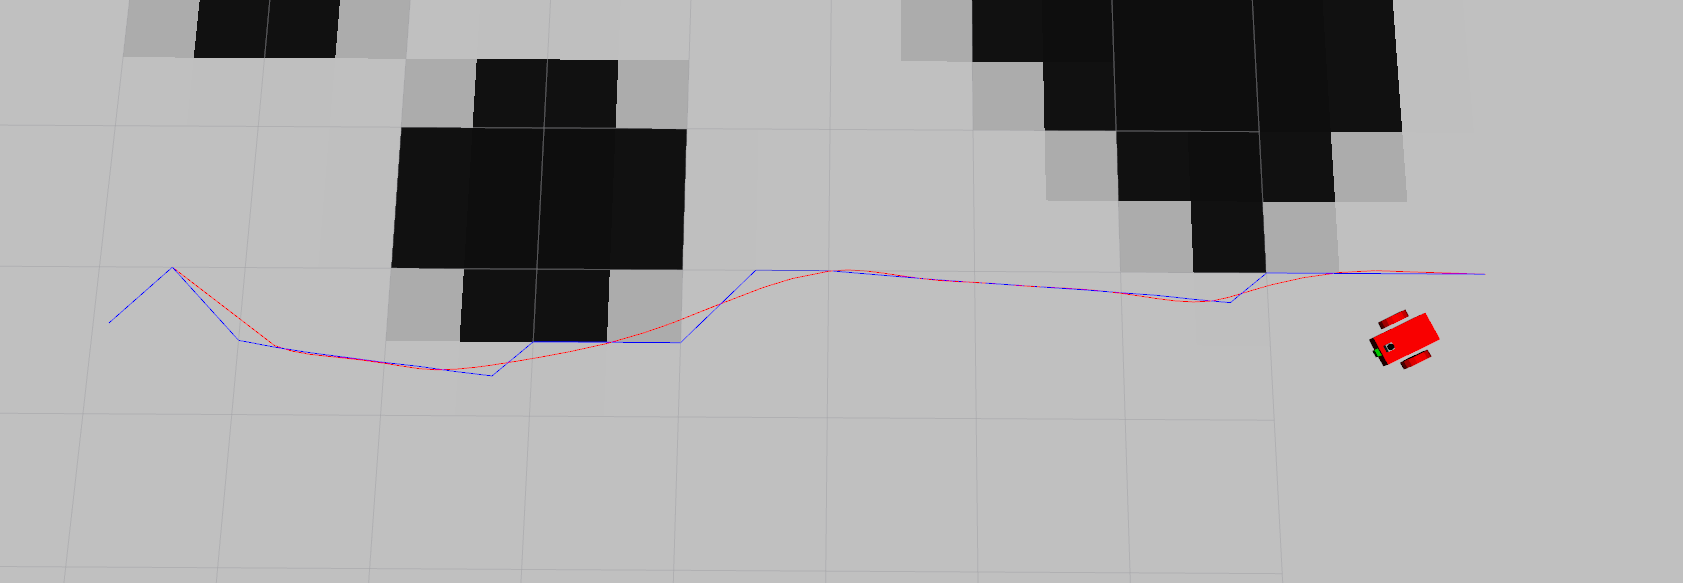
\includegraphics[width=16cm]{pic/preizkus_k.png}
	\caption{Prikaz delovanja algoritma glajenja poti.}
	\label{fig:slika7}
\end{figure}

Ugotovili smo, da je algoritem primeren za reševanje problema glajenja poti. Pri tem pa je potrebno omeniti, da je kvaliteta končne, gladke poti odvisna od najdenih optimalnih parametrov. Pogoj za uspešno glajenje je tudi stanje osnovne grobe poti, glajenje je namreč problematično ob prisotnosti zelo velikih kotov med odseki poti (okolica $90^{\circ}$). Končna pot je takem primeru neuporabna.

Problemi bazične izvedbe algoritma tičijo v težko predstavljivih parametrih, kar povzroča težave pri njihovemu nastavljanju s strani končnega uporabnika. Poleg tega pa se ustreznost paramterov spreminja nelinearno z dimenzijo problema. Kot smo ugotovili je ta problem mogoče rešiti z aplikacijo optimizacijskih agloritmov, kjer iščemo paramtere tako, da nam ti optimirajo ustrezno kriterijsko funkcijo, ki je odraz kvalitete poti. V našem primeru smo to storili tako, da smo poskušali pridobiti ustrezno slabo pot iz navigacijskega algoritma ter na njeni osnovi iskali optimalne parametre. Takšna rešitev je ustrezna za primer kjer se inicializacija vozila izvaja v okolju s prisotnostjo ovir. Če  v okolici avtonomnega vozila ovir ni, je pridobitev grobe poti iz navigacijskega algortma nemogoča in tako je iskanje ustreznih paramterov neizvedljivo.

Omenjeni problem iskanja paramterov bi bilo moč rešiti tako, da se optimizacija izvaja na osnovi grobe poti, polja točk, ki je programu vedno na voljo (polje v programu ali tekstovna datoteka) in se ga pred iskanjem parametrov skalira v skladu z dimenzijo problema. Ustrezni skalirni faktor bi bilo moč najti z še eno, predhodno optimizacijo, na primer z minimizacijo napake med povprečinimi razdaljami shranjene grobe poti ter neke poti navigacijskega okolja avtonomnega vozila. Skalirni faktor bi bilo mogoče določiti tudi na podlagi informacije o ločljivosti zemljevida vrednosti. Iskanje ustreznih paramterov bi lahko poskusili tudi na analitičen način.

Načrti v prihodnosti bi lahko obsegali preizkus na pravemu vozilu, prepis vozlišča v hitrejši jezik C++, ki ga ROS podpira poleg Python-a. Na sliki \ref{fig:slika7} vidimo, da je glajenje poti dokaj lokalno ali z drugimi besedami, obstaja bolj neposredna pot od vozila do cilja. Za izboljšavo omnejenega opažanja bi lahko preizkusili uporabo lokalnih paramterov glajenja oziroma takšno glajenje, kjer ima vsaka točka glajenja poti svoj set paramterov. Pri tem problemu pa se je smiselno vprašati ali je to problem domene glajenja poti ali problem tvorjenja globalne poti v okviru navigacijskega sklada.